\documentclass[12pt,a4paper]{amsart}
\usepackage[utf8]{inputenc}
\usepackage{amsmath}
\usepackage{amsfonts}
\usepackage{amssymb}

\usepackage[all,cmtip]{xy}

\usepackage{hyperref}

\usepackage{float}
\usepackage{subfig}


%\usepackage[dvipdfmx]{graphicx}
\usepackage{graphicx}
\usepackage{caption}
%\usepackage[nobysame, alphabetic]{amsrefs}
%\usepackage{here}
%\usepackage{showkeys}
\newcommand{\modif}{$\clubsuit$}
\newtheorem{thm}{Theorem}[section]
\newtheorem{defn}[thm]{Definition}
\newtheorem{coro}[thm]{Corollary}
\newtheorem{prop}[thm]{Proposition}
\newtheorem{lem}[thm]{Lemma}
%\theoremstyle{definition}
\newtheorem{rmk}[thm]{Remark}
\newtheorem{cond}[thm]{Condition}

%CB defs
\def\rh{\phi_h}
\def\rv{\phi_v}

\def\HH{\mathbb{H}}
\def\GG{\mathbb{G}}
\def\dHH{\partial \mathbb{H}}
\def\hd{\hat{\delta}}
\def\ha{\hat{\alpha}}
\def\haa{\ha \cup \{\alpha^+,\alpha^-\}}

\def\im{\mathrm{Im}\,}
\def\re{\mathrm{Re}\,}
\def\oo{\HH / \Gamma_0(2)} 
\def\ooo{\HH / \Gamma_0(3)} 
\def\g2{\Gamma(2)}
\def\go2{\Gamma_0(2)}
\def\ah{\Gamma_0^t(2)}
\def\oot{\HH / \ah} 
\def\xx{\HH/\g2}


\def\ZZ{\mathbb{Z}}
\def\CC{\mathbb{C}}
\def\RR{\mathbb{R}}
\def\QQ{\mathbb{Q}}
\def\NN{\mathbb{N}}

\def\qqq{\mathbb{Q} \cup \{\infty\}}

\def\tt{\Sigma_{1,1}}

\def\fp{\mathbb{F}_p}
\def\aut{\text{Aut}(\F2)}
\def\gl2{\mathrm{GL}(2, \ZZ)}
\def\sl2{\mathrm{SL}(2, \ZZ)}
\def\slc{\mathrm{SL}(2, \CC)}

\def\oi{\Gamma.\{i\}}

\def\gg{\mathcal{G}_n}
\def\ggp{\mathcal{G}_p}

\def\isom{\mathrm{isom}(\HH)}

\def\isomH{\text{isom}^+(\HH)}
\def\tr{\text{tr\,}}


\def\GI{\mathbb{Z}[i]}
\def\hc{\CC \setminus \GI}



\title{Pythagorean triples}

 % \author[Vlad]{Vlad Sergesciu}
\address{Institut Fourier 100 rue des maths, BP 74, 38402 St Martin d'H\`eres cedex, France}
\email{mcshane at univ-grenoble-alpes.fr}


\begin{document}

\maketitle

\section{Introduction}

A \textit{Pythagorean triple} is a triple of integers $(a,b,c)$ such
that $$a^2 + b^2 = c^2.$$
The most famous example is the so-called \textit{egyptian triple}
$(3,4,5)$ which is \textit{a priori} the ``smallest'' Pythagorean triple.	
The set of Pythagorean triples is infinite, and it is a classical problem to find all Pythagorean triples. 
It is useful to define the notion of \textit{primitive Pythagorean
triple}, which is a Pythagorean triple $(a,b,c)$ such that
the three integers have no common divisor greater than 1.
Evidently, any Pythagorean triple can be written as a multiple of a primitive Pythagorean triple.
In fact, the set of primitive Pythagorean triples 
forms a single orbit under the action of a group of transformations the orthognal group $O(2,1;\ZZ)$ on the Minkowski space $\mathbb{R}^{2,1}$.
This is because every Pythagorean triple is an integer point on the
\textit{light cone} of Minkowski space: 
$$ \{ (x,y,z) \in \mathbb{R}^3 \mid -x^2 - y^2 + z^2 = 0 \}.$$
We note that the ``smallest" integer point on the light cone is not
$(3,4,5)$, but rather $(1,0,1)$ or $(0,1,1)$.
Of course, these two points correspond to degenerate Pythagorean triangles i.e. triangles of area zero.

\section{Euclid's parameterization}


The Pythagorean triples that are relatively prime (called the primitive triples) have
the elementary and beautiful characterization as integers
due to Euclid:
$$(a,b,c) = (m^2 - n^2, 2mn, m^2 + n^2)$$
where $m$ and $n$ are coprime integers of opposite parity and $m > n > 0$.
Another way to think of this is
that $c$ factors over the Gaussian integers $\mathbb{Z}[i]$ 
as 
$$c = (m+ni)(m-ni),$$ 
where $m$ and $n$ are coprime integers of opposite parity,
that is exactly one is odd and the other is even
so it follows that $c= m^2 + n^2$ is odd,
and $a$ is the real part of the product and $b$ is the imaginary part of the product.

\section{Alperin's approach}


Alperin's approach \cite{alperin} to enumerating primitive Pythagorean triples is based on a
correspondence between the triples a subset of the nilpotent cone  matrices $\mathcal{N}_2$. 


\begin{figure}[hb]
\begin{center}
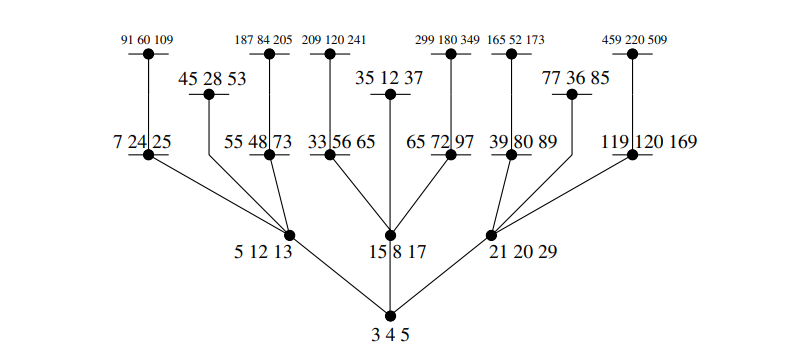
\includegraphics[scale=.5]{alperin_tree.png} 
\end{center}
\caption{Alperin's tree of Pythagorean triples.}
\label{farey diagram}
\end{figure}


\begin{lem}
 \textit{An integer matrix $X$ satisfies $X^2 = 0$ if and only if $X$ has the form}
\[
	X 
	= \begin{pmatrix} x & y \\ z & -x \end{pmatrix}
	= \begin{pmatrix}
mn & -n^2 \\
m^2 & -mn
\end{pmatrix}
	= \begin{pmatrix} n \\ m \end{pmatrix} \begin{pmatrix} m & -n 
\end{pmatrix}	
\]

\textit{for integers $x$, $y$, and $z$ such that $x^2 + yz = 0$.}
\end{lem}

The group $\sl2$ acts on the nilpotent cone $\mathcal{N}_2$ by
conjugation.






\begin{table}[h]
% \centering
\renewcommand{\arraystretch}{2}
\begin{tabular}{|c|c|c|}
\hline
\multicolumn{3}{|c|}{\textbf{Magic Correspondence}} \\
\hline
 & Minkowski space $\mathbb{R}^{2,1}$ & Traceless $2 \times 2$ matrices \\
\hline
Main object & 
$\mathbf{v} = (x, y, z)$ & 
$\tilde{\mathbf{v}} = \sum v^i \sigma_i = \frac{1}{2}
\begin{pmatrix} -y & x+z \\ x-z & y \end{pmatrix}$ \\
\hline
Norm & 
$\|\mathbf{v}\| = -x^2 - y^2 + z^2$ & 
$\|\mathbf{v}\| = 4 \det \tilde{\mathbf{v}}$ \\
\hline
Action & 
$\mathbf{v}' = A\mathbf{v}$,\, \newline ($A \in O(2,1;\mathbb{Z})$) & 
$\tilde{\mathbf{v}}' = \tilde{A} \tilde{\mathbf{v}} \tilde{A}^*$,\, \newline ($\tilde{A} \in SL^{\pm}(2,\mathbb{Z})$) \\
\hline
Minkowski scalar product & 
$\mathbf{v} \cdot \mathbf{w} = \mathbf{v}^T G \mathbf{w}$ & 
$\mathbf{v} \cdot \mathbf{w} = -2 \mathrm{Tr}\,\tilde{\mathbf{v}} \tilde{\mathbf{w}}$ \\
\hline
The $i$th coefficient & 
$v^i = \mathbf{v} \cdot \mathbf{e}_i$ & 
$v^i = -\det \sigma_i \cdot \mathrm{Tr}(\tilde{\mathbf{v}} \sigma_1)$ \\
\hline
\end{tabular}
\caption{Correspondence between Minkowski space and traceless $2 \times 2$ matrices.}
\end{table}


\begin{table}[h]
% \centering
\renewcommand{\arraystretch}{2}
\begin{tabular}{|l|l|}
% \toprule
\textbf{Hyperbolic Geometry} & \textbf{Algebra/Number Theory} \\
\hline
horocycle & nonzero vector $(p,q) \in \mathbb{R}^2$ \\
	  % & &\\
\hline
geodesic & indefinite binary quadratic form $f$ \\
point & definite binary quadratic form $f$ \\
signed distance between horocycles & $2 \log \left| \det \begin{pmatrix} p_1 & p_2 \\ q_1 & q_2 \end{pmatrix} \right|$ \\
signed distance between horocycle & $\log \left( \dfrac{f(p,q)}{\sqrt{|\det f|}} \right)$ \\
% and geodesic/point & \\
% ideal triangulation of the modular torus & Markov triple \\
% \bottomrule
\end{tabular}
\caption{Correspondence between hyperbolic geometry and algebra/number theory.}
\end{table}

\thebibliography{99}

\bibitem{aigner2}
Aigner M., Ziegler G.M.  
\textit{Representing numbers as sums of two squares.} In: Proofs from THE BOOK. Springer, Berlin, Heidelberg. (2010)

\bibitem{conway}
Conway, J. H. and Guy, R. K. \textit{Farey Fractions and Ford
Circles.} The Book of Numbers. New York: Springer-Verlag, pp. 152-154, 1996.

\bibitem{dolan}
Dolan, S., 
\textit{A very simple proof of the two-squares theorem.}
The Mathematical Gazette, 106(564), 511-511. (2021) doi:10.1017/mag.2021.120

\bibitem{elsholtz}
Elsholtz C.A 
\textit{Combinatorial Approach to Sums of Two Squares and Related Problems.}
 In: Chudnovsky D., Chudnovsky G. (eds) Additive Number Theory. Springer, New York, NY.
 (2010) 


\bibitem{ford}
Ford, L. R.,  \textit{Fractions.} Amer. Math. Monthly, 45, (9), 586–601 (1938).



%\bibitem{haas1}
%
%Andrew Haas. 
%\textit{Diophantine approximation on hyperbolic Riemann surfaces.} Acta Math. 156 33 - 82, 1986.

%\bibitem{haas2}
%\textit{The geometry of Markoff forms.} Number Theory, New York
%pp 232-244
%Lecture notes in math 1240, 1988


\bibitem{heath}
Heath-Brown, Roger. 
\textit{ Fermat’s two squares theorem.} Invariant (1984) 

%\bibitem{huang}
%Yi Huang
%\textit{Moduli Spaces of Surfaces}
%Ph.D. Thesis, The University of Melbourne (2014)



\bibitem{vlad}
Greg McShane, Vlad Sergiescu,
\textit{Geometry of Fermat's sum of squares}
\url{https://macbuse.github.io/squares.pdf}

\bibitem{macbuse}
Github repo FAREY DIAGRAM \url{https://github.com/macbuse/FAREY_DIAGRAM}

\bibitem{bob}
R. C. Penner, 
\textit{The decorated Teichmueller space of punctured surfaces}, 
Communications in Mathematical Physics 113 (1987), 299–339.


% \bibitem{north}
% Northshield, Sam. 
% \textit{A Short Proof of Fermat’s Two-square Theorem.} The American Mathematical Monthly. 127. 638-638. (2020). 

\bibitem{serre}
J-P. Serre,
\textit{A Course in Arithmetic},
Graduate Texts in Mathematics,
Springer-Verlag New York
1973


% \bibitem{series}
% Series, C. (1985), 
% \textit{The Modular Surface and Continued Fractions. Journal of the London} Mathematical Society, s2-31: 69-80. 

\bibitem{springborn1}
B. Springborn. The hyperbolic geometry of Markov’s theorem on Diophantine
approximation and quadratic forms. Enseign. Math., 63(3-4):333–373, 2017.

\bibitem{springborn2}
Boris Springborn,
\textit{The worst approximable rational numbers}
\url{https://arxiv.org/abs/2209.15542}



\bibitem{zagier}
D. Zagier,
 \textit{A one-sentence proof that every prime p = 1 (mod 4) is a sum of two squares}, 
 American Mathematical Monthly, 97 (2): 144

 \bibitem{copilot}
 Github Copilot \url{https://copilot.github.com/}

 \bibitem{vim_copilot}
Tim Pope, copilot.vim \url{https://github.com/github/copilot.vim}
 

\bibitem{vim}
Daniel V. Mathews,
\textit{Spinors and horospheres}
\url{https://arxiv.org/abs/2308.09233}

\bibitem{kocik1}
Jerzy Kocik,
\textit{Clifford Algebras and Euclid's Parameterization of Pythagorean Triples},
Advances in Applied Clifford Algebras 17 (2007), 71-93.
\url{https://arxiv.org/abs/1201.4418}

\bibitem{hall}
 A. Hall, 
 Genealogy of Pythagorean triads, 
 Mathematical Gazette, LIV, No. 390
(1970), 377–379.

\bibitem{hall2}
Keith Conrad
Pythagorean descent
\url{https://kconrad.math.uconn.edu/blurbs/linmultialg/descentPythag.pdf}

\bibitem{alperin}
 R. C. Alperin, 
 The Modular Tree of Pythagoras,
 Amer. Math. Monthly 112 (2005), 807–816
 \url{https://web.archive.org/web/20231014013915/http://www.math.sjsu.edu/%7Ealperin/pt.pdf}

 \bibitem{lee}
H. Lee Price
 The Pythagorean Tree: A New Species
 \url{https://arxiv.org/abs/0809.4324}

\end{document}
